
\section{Introduction to Advanced Design Patterns} \label{sec:advanced-intro}

Cardano smart contracts are powerful, but writing efficient and scalable on-chain code requires thinking carefully about resource constraints, data structures, and contract architecture. In this chapter we explore advanced design patterns from the Anastasia Labs open-source library \texttt{aiken-design-patterns}\footnote{\url{https://github.com/Anastasia-Labs/aiken-design-patterns}}, a collection of battle-tested patterns for building production-grade Cardano smart contracts.

These patterns address real challenges that developers face when moving beyond simple validators: how to handle unbounded data sets, how to reduce on-chain computation costs, and how to structure complex multi-contract systems efficiently.

% =============================================================================
\section{Linked List as Infinite Array in eUTxO} \label{sec:linked-list}
% =============================================================================

\subsection{The Array Problem in Blockchain}

Computers and programmers have always had an issue with arrays: should the size be defined upfront or should it grow dynamically? In traditional programming, dynamic arrays require careful memory management -- allocating new space and freeing old memory. On a blockchain, this problem takes a different character.

In Cardano, the list type from the Plutus standard library allows elements to be added without specifying a size upfront, which is convenient. However, every transaction has a strict limit on the amount of data it can read and process. As soon as we want to store a list in a datum, we must accept that we cannot work with an arbitrarily large collection within a single transaction.

The Cardano ledger defines list operations in the \texttt{plutus-tx} library. A simplified view of how lists behave on-chain is shown below -- note that traversing the entire list within a single transaction quickly becomes infeasible for large collections:

\begin{lstlisting}[language=haskell, caption=List operations in Plutus Tx (github.com/IntersectMBO/plutus)]
-- Source: plutus-tx/test/List/Spec.hs
-- Lists in Plutus Tx are standard Haskell-like types

-- A simple list of integers
example :: [Integer]
example = [1, 2, 3, 4, 5]

-- Traversal is O(n) -- expensive in on-chain execution
sumList :: [Integer] -> Integer
sumList []     = 0
sumList (x:xs) = x + sumList xs

-- Plutus Tx enforces an execution budget.
-- A list with thousands of entries cannot be
-- traversed in a single transaction.
\end{lstlisting}

The key constraint is: \textbf{within a single transaction, you cannot process an arbitrarily large list}. The on-chain execution budget (CPU and memory units) is fixed. A list with thousands of elements stored in one datum cannot be traversed in one transaction.

\subsection{Linked Lists in eUTxO}

The solution is to use UTxOs themselves as list elements. Instead of storing an entire array in a single datum, each element becomes its own UTxO. The datum of each UTxO contains a pointer (the transaction output reference) to the next element, forming a chain -- a \textbf{linked list}.

\begin{figure}[ht]
    \centering
    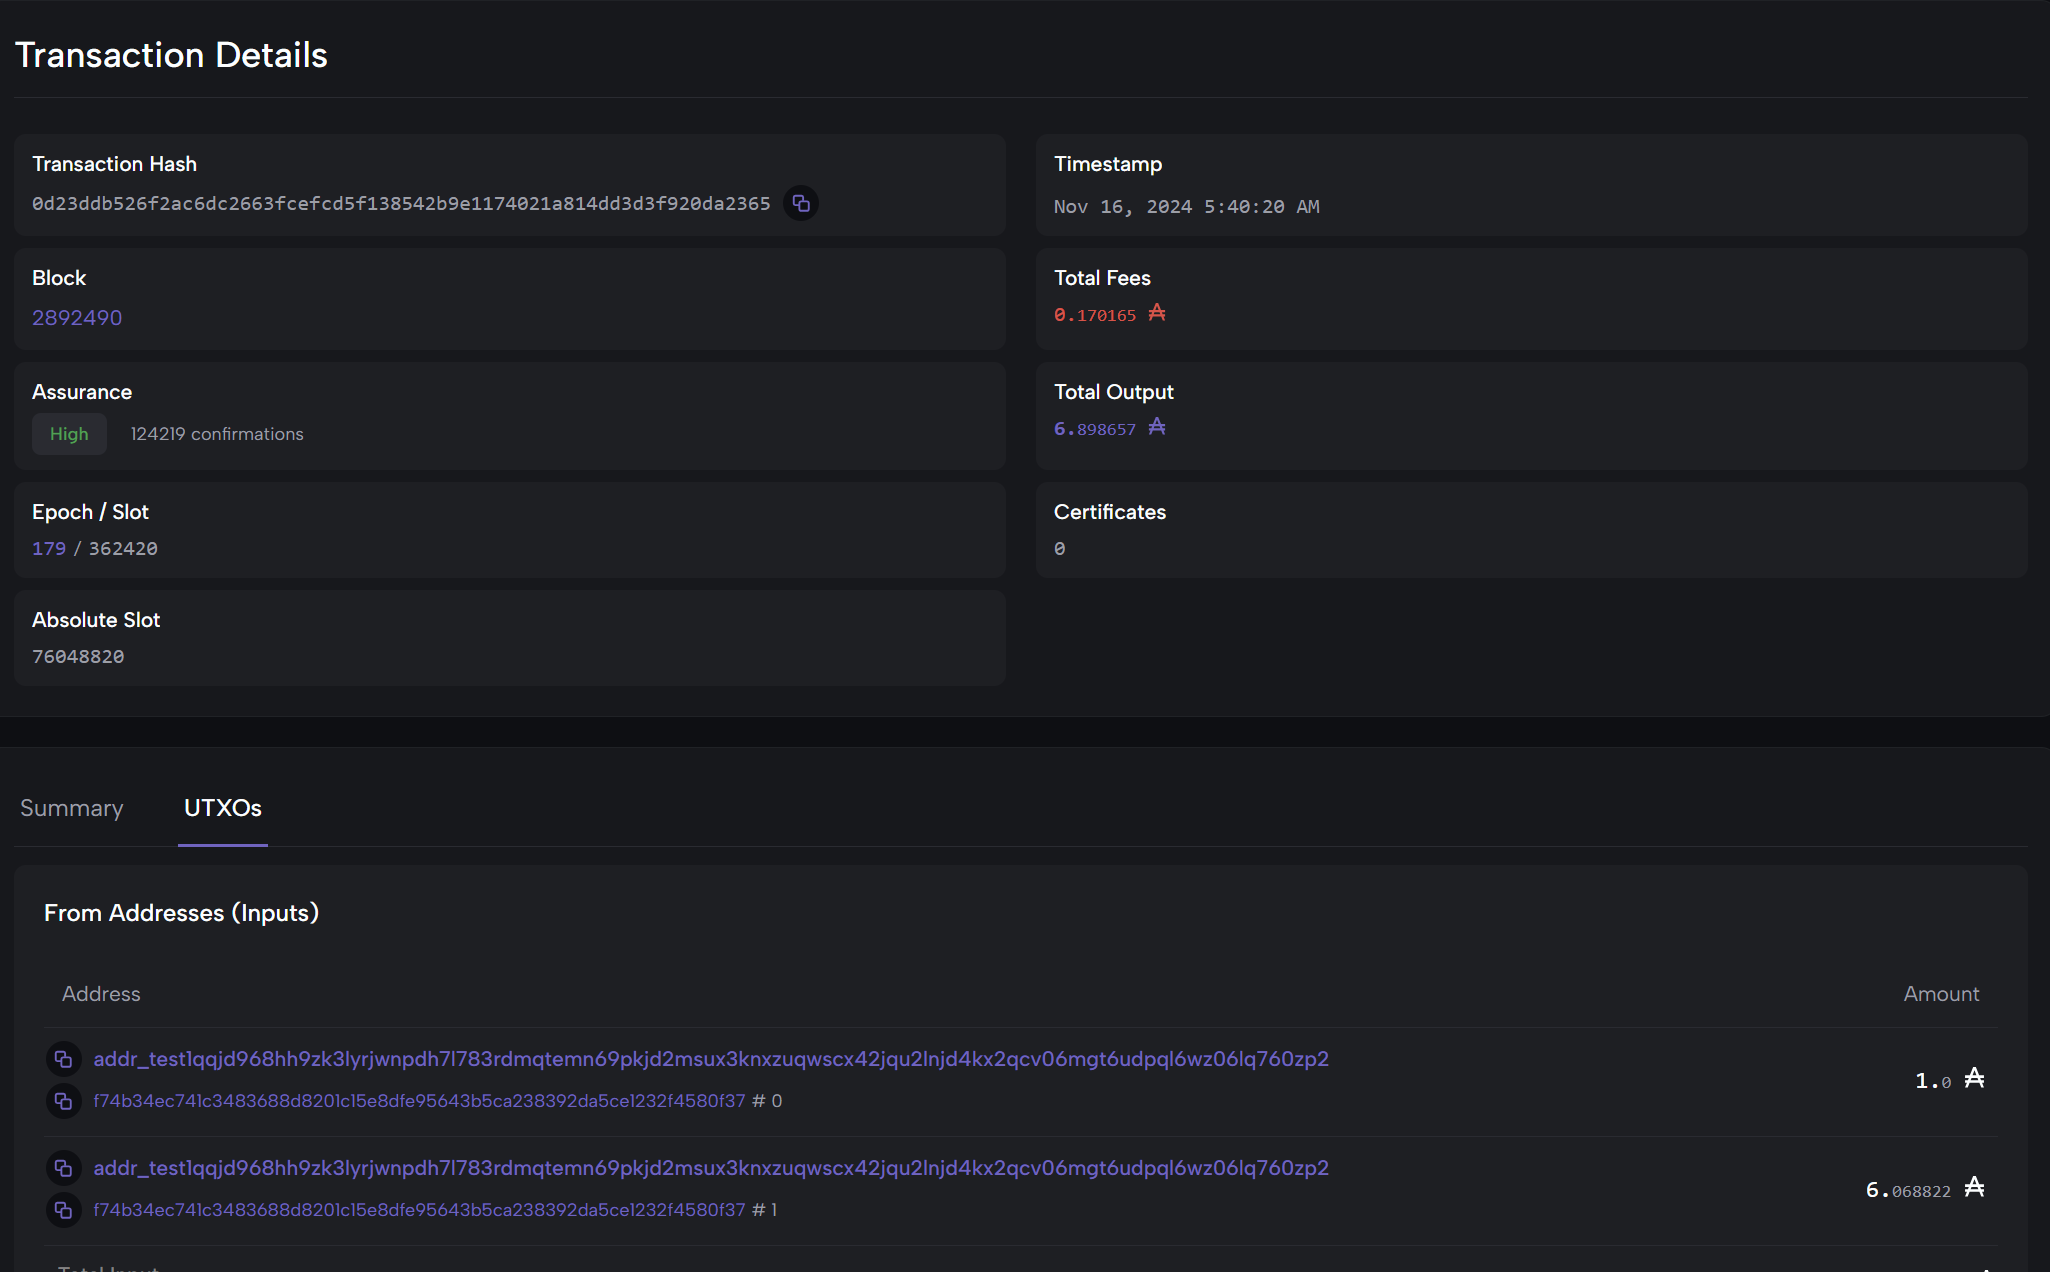
\includegraphics[width=0.8\textwidth]{images/lock.png}
    \caption{Each node in the linked list is a separate UTxO, pointing to the next}
    \label{fig:linked-list}
\end{figure}

The structure of each node looks like this in Aiken:

\begin{lstlisting}[language=haskell, caption=Linked List Node Datum in Aiken]
// From: github.com/Anastasia-Labs/aiken-design-patterns

pub type NodeKey {
  Key(ByteArray)
  Empty
}

pub type LinkedListNode {
  key: NodeKey,
  next: NodeKey,
}
\end{lstlisting}

Each node holds a \texttt{key} (its own identifier, often derived from a credential or token name) and a \texttt{next} pointer to the following node. The last node in the list has \texttt{next = Empty}.

\subsection{Advantages of the eUTxO Linked List}

This pattern offers several important benefits:

\begin{itemize}
    \item \textbf{Unbounded size:} The list can grow indefinitely, limited only by the ADA required to create each UTxO (at minimum ADA values, 10,000 elements would require at least 10,000 ADA).
    \item \textbf{Efficient membership proofs:} Instead of searching the entire list on-chain, you locate the relevant element off-chain and prove its inclusion (or exclusion) by providing it as a reference input. The contract validates the proof without traversing the list.
    \item \textbf{Parallelism:} Multiple transactions can interact with different elements simultaneously, since each element is an independent UTxO.
\end{itemize}

\subsection{Proving Membership Off-Chain}

The real power of this pattern is in membership proofs. To check whether an element belongs to the list, you do \textbf{not} traverse the entire chain on-chain. Instead:

\begin{enumerate}
    \item Off-chain code finds the node containing the element.
    \item The transaction provides that UTxO as a reference input.
    \item The validator confirms that the node's key matches what is expected and that the node belongs to the list (verified by checking the validator address and the node structure).
\end{enumerate}

This shifts expensive O(n) traversal off-chain, making on-chain validation O(1).

\begin{lstlisting}[language=haskell, caption=Checking List Membership in Aiken]
use aiken/collection/list
use cardano/transaction.{Input}

// Verify that a node with `target_key` exists
// among the reference inputs at the list address
fn has_member(
  reference_inputs: List<Input>,
  list_address: Address,
  target_key: ByteArray,
) -> Bool {
  list.any(reference_inputs, fn(input) {
    let is_at_list_address =
      input.output.address == list_address
    let has_correct_key = when input.output.datum is {
      InlineDatum(raw_datum) -> {
        expect node: LinkedListNode = raw_datum
        node.key == Key(target_key)
      }
      _ -> False
    }
    is_at_list_address && has_correct_key
  })
}
\end{lstlisting}

\subsection{When to Use Linked Lists}

Linked lists are ideal for:
\begin{itemize}
    \item \textbf{Allowlists and blocklists:} Storing a set of authorized addresses or blacklisted entities.
    \item \textbf{Staking position tracking:} Keeping a record of staking positions in a protocol where new entries can be added at any time.
    \item \textbf{Order books:} Maintaining a sorted list of open orders in a DEX.
\end{itemize}

\subsection{Merkle Patricia Forestry}

When you need to store a large amount of \textit{data} (rather than a large \textit{count} of elements) and compress it into a single hash, Merkle Patricia tries are a better fit than linked lists. The \texttt{merkle-patricia-forestry} library provides an Aiken-compatible implementation:

\begin{center}
\url{https://github.com/aiken-lang/merkle-patricia-forestry}
\end{center}

A Merkle Patricia trie stores all data off-chain, compressing everything into a single root hash stored on-chain. Proofs of inclusion are logarithmic in size, making them efficient to verify in a transaction. The trade-off is that the actual data must be stored somewhere (IPFS, a server, or another off-chain system) -- the on-chain hash alone is not enough to reconstruct the data.

% =============================================================================
\section{Merklized Validators for Scalable Contracts} \label{sec:merklized-validators}
% =============================================================================

\subsection{The Monolithic Validator Problem}

If you have built smart contracts on Cardano, you have probably encountered this frustration: every time a transaction interacts with your contract, the \textit{entire} script must be loaded into the transaction evaluation context -- even if only a tiny fraction of its logic is relevant to that specific interaction.

Consider a marketplace contract that supports two actions:
\begin{itemize}
    \item \textbf{Buy:} A buyer purchases a listed NFT.
    \item \textbf{Delist:} The seller removes their listing.
\end{itemize}

When a seller delists an NFT, the transaction still loads and evaluates the Buy logic, the royalties calculation, and every other handler -- even though none of it is needed. This wastes execution units and increases fees.

There are two deeper problems with monolithic validators:

\begin{enumerate}
    \item \textbf{Non-upgradable code:} Smart contracts on Cardano are immutable. If you discover a bug in the Buy handler, you must redeploy the \textit{entire} marketplace, migrate all existing listings, and re-audit the whole contract.
    \item \textbf{Script size limits:} As contracts grow in complexity, they can approach or exceed the maximum script size that can be included in a transaction reference input.
\end{enumerate}

\subsection{The Merklized Validator Pattern}

The solution is to decompose the monolithic contract into a family of smaller contracts:

\begin{itemize}
    \item \textbf{A container (spend) validator} that holds the assets (e.g., listed NFTs). This contract is minimal -- it only verifies that the correct action validator was executed as part of the transaction.
    \item \textbf{Action validators} implemented as \texttt{REWARD} (withdrawal) scripts. Each action (Buy, Delist, etc.) is its own script. These scripts are executed only when their specific action is triggered.
\end{itemize}

The key insight is that \textbf{withdrawal scripts} (\texttt{REWARD} purpose) in Cardano are executed once per transaction, regardless of how many UTxOs they authorize. This means:

\begin{itemize}
    \item When a buyer purchases 10 NFTs at once, the Buy script runs \textit{once}, not 10 times.
    \item The Delist logic is never loaded during a Buy transaction.
    \item If a bug is found in the Buy script, only the Buy script needs to be redeployed and audited.
    \item Furthermore, the fix can be audited in isolation -- a much smaller scope than the entire marketplace.
\end{itemize}

\subsection{Implementing the Pattern in Aiken}

The container validator checks that the appropriate action script has been executed by verifying its presence in the transaction's withdrawals:

\begin{lstlisting}[language=haskell, caption=Container Validator (Spend) in Aiken]
// From: github.com/Anastasia-Labs/aiken-design-patterns

use aiken/collection/dict
use cardano/transaction.{Transaction}
use cardano/address.{Inline, Script}

pub type MarketplaceRedeemer {
  Buy
  Delist
}

validator marketplace(
  buy_script_hash: ByteArray,
  delist_script_hash: ByteArray,
) {
  spend(
    _datum: Option<Data>,
    redeemer: MarketplaceRedeemer,
    _utxo: OutputReference,
    tx: Transaction,
  ) {
    let required_script = when redeemer is {
      Buy    -> buy_script_hash
      Delist -> delist_script_hash
    }
    // Verify the action script was executed
    // by checking it appears in withdrawals
    dict.has_key(
      tx.withdrawals,
      Inline(Script(required_script)),
    )
  }

  else(_) { fail }
}
\end{lstlisting}

The action scripts are \texttt{REWARD} validators that contain the actual business logic. For example, the Buy action script validates that the correct payment is made to the seller:

\begin{lstlisting}[language=haskell, caption=Buy Action Script (Reward) in Aiken]
validator buy_action {
  withdraw(_redeemer: Data, _account: Credential,
           tx: Transaction) {
    // All buy logic lives here:
    // - NFT transferred to buyer
    // - Seller receives correct payment
    // - Royalties paid if applicable
    // - Marketplace fee collected
    validate_purchases(tx)
  }

  else(_) { fail }
}
\end{lstlisting}

\subsection{Benefits Summary}

\begin{table}[ht]
\centering
\small
\begin{tabular}{|l|p{4.5cm}|p{4.5cm}|}
\hline
\textbf{Property} & \textbf{Monolithic Validator} & \textbf{Merklized Validator} \\ \hline
Script size & Grows with every new feature & Container stays minimal \\ \hline
Fee per action & All logic loaded every time & Only relevant action loaded \\ \hline
Upgradeability & Redeploy everything & Redeploy only changed action \\ \hline
Audit scope & Entire contract on every fix & Only the modified action script \\ \hline
Multi-UTxO efficiency & Script runs per UTxO & Reward script runs once per tx \\ \hline
\end{tabular}
\caption{Monolithic vs.\ merklized validator architectures}
\end{table}

% =============================================================================
\section{Special Tips and Tricks} \label{sec:tips-tricks}
% =============================================================================

\subsection{Separating Spend and Mint Logic}

A common mistake when writing Cardano smart contracts is combining \texttt{spend} and \texttt{mint} logic into a single validator. While Cardano supports multi-purpose validators, this pattern introduces an avoidable inefficiency.

\subsubsection{The Self-Referential Hash Problem}

Imagine a contract that, in order to authorize spending a UTxO, checks whether a specific NFT is present in that UTxO -- an NFT whose minting policy is the contract's \textit{own} script hash. This creates a bootstrapping problem:

\begin{itemize}
    \item The contract needs to know its own hash to identify the NFT's policy.
    \item The hash of a script depends on its compiled bytecode.
    \item Any reference to the hash inside the script changes the bytecode, which changes the hash -- a circular dependency.
\end{itemize}

In practice, the script can introspect its own execution context to derive its hash at runtime, but this computation is expensive and must be repeated for every UTxO being spent. The cost multiplies quickly when many UTxOs are consumed in a single transaction.

\begin{lstlisting}[language=haskell, caption=Costly self-referential hash in a combined validator]
// Inefficient: computing own hash for every spend
validator combined {
  spend(datum, redeemer, own_ref, tx) {
    // Expensive: must find own input to get own address
    expect Some(own_input) =
      transaction.find_input(tx.inputs, own_ref)
    let own_address = own_input.output.address
    // ... derive own policy from own_address, then
    // check that the NFT with that policy is present
    True
  }

  mint(redeemer, policy_id, tx) {
    // ... minting logic
    True
  }
}
\end{lstlisting}

\subsubsection{The Solution: Two Dedicated Contracts}

The solution is to use two separate contracts:

\begin{enumerate}
    \item \textbf{A minting policy} dedicated to the NFT. Its hash is the policy ID and is fixed at compile time.
    \item \textbf{A spend validator} that receives the minting policy hash as a \textit{parameter}. Since the policy hash is now a fixed parameter (not self-derived), the spend validator never needs to compute its own hash.
\end{enumerate}

\begin{lstlisting}[language=haskell, caption=Clean split: separate minting policy and spend validator]
// 1. The NFT minting policy is a dedicated contract
validator nft_policy {
  mint(_redeemer: Data, _policy_id: PolicyId,
       tx: Transaction) {
    // ... minting conditions (e.g. one-shot minting)
    True
  }
  else(_) { fail }
}

// 2. The spend validator receives the policy as a
//    parameter -- no runtime hash derivation needed
validator marketplace(nft_policy_id: PolicyId) {
  spend(datum, redeemer, _own_ref, tx) {
    // Direct and cheap: policy_id is already known
    let nft_present = assets.quantity_of(
      utxo_value,
      nft_policy_id,
      expected_token_name,
    ) == 1
    nft_present
  }
  else(_) { fail }
}
\end{lstlisting}

This split makes the spend validator cheaper to execute (no runtime hash derivation) and conceptually cleaner -- each contract has a single, well-defined responsibility.

\subsection{Settings UTxO Pattern}

As your protocol evolves, you will encounter parameters that may need to change without redeploying your core contracts: admin addresses, fee percentages, whitelisted oracles, authorized script hashes, and so on.

\subsubsection{The Problem with Hardcoded Parameters}

If these values are hardcoded as validator parameters, updating them means deploying a new version of the contract and migrating all existing state. This is expensive, disruptive, and error-prone.

\subsubsection{The Settings UTxO}

The Settings UTxO pattern introduces a special UTxO held at a dedicated settings validator address. Its inline datum contains all mutable protocol parameters:

\begin{lstlisting}[language=haskell, caption=Settings Datum Structure in Aiken]
pub type ProtocolSettings {
  admin: Address,
  fee_percent: Int,
  whitelisted_oracles: List<ByteArray>,
  authorized_scripts: List<ByteArray>,
  version: Int,
}
\end{lstlisting}

Core validators reference this settings UTxO as a \textbf{reference input} (read-only, no consumption needed). When parameters need updating, only the settings UTxO is modified -- the core contracts remain unchanged and do not need to be redeployed.

\begin{lstlisting}[language=haskell, caption=Reading Settings from a Reference Input]
use aiken/collection/list
use cardano/transaction.{Input}

fn get_settings(
  reference_inputs: List<Input>,
  settings_address: Address,
) -> ProtocolSettings {
  expect Some(settings_input) =
    list.find(reference_inputs, fn(input) {
      input.output.address == settings_address
    })
  expect InlineDatum(raw) = settings_input.output.datum
  expect settings: ProtocolSettings = raw
  settings
}
\end{lstlisting}

\subsubsection{Governance of the Settings UTxO}

The settings validator itself should be simple but secure:

\begin{itemize}
    \item \textbf{Admin-only updates:} Only the admin address recorded in the current settings can authorize an update transaction.
    \item \textbf{Version enforcement:} The new datum must carry an incremented version number to prevent replay attacks.
    \item \textbf{Continuity check:} The updated settings must be sent back to the same settings validator address, ensuring the UTxO remains under protocol control.
\end{itemize}

This pattern gives your protocol a lightweight, upgradeable configuration layer without requiring any smart contract redeployment.

% =============================================================================
\section{Key Takeaways} \label{sec:advanced-takeaways}
% =============================================================================

\begin{itemize}
    \item \textbf{Linked lists} use UTxOs as nodes, enabling unbounded data structures on Cardano. Off-chain code computes membership proofs; on-chain validators verify them in O(1) time. The cost is on-chain storage: each node requires a UTxO with minimum ADA.
    \item \textbf{Merkle Patricia tries} compress large data sets into a single on-chain hash. They are ideal when the data itself can live off-chain and you only need efficient membership proofs.
    \item \textbf{Merklized validators} decompose monolithic contracts into a minimal container and focused action scripts (reward validators). This reduces fees, enables partial upgrades, and limits audit scope to only changed components.
    \item \textbf{Splitting spend and mint} into separate contracts eliminates expensive self-referential hash computation and gives each contract a single responsibility. The minting policy hash becomes a fixed parameter of the spend validator.
    \item \textbf{Settings UTxOs} provide a protocol configuration layer that can be updated without redeploying core validators, using reference inputs to share parameters across all contracts in the protocol.
    \item All of these patterns are available as open-source building blocks in the Anastasia Labs \texttt{aiken-design-patterns} repository: \url{https://github.com/Anastasia-Labs/aiken-design-patterns}
\end{itemize}
